\documentclass{article}

\usepackage{arxiv}

\usepackage[utf8]{inputenc} % allow utf-8 input
\usepackage[T1]{fontenc}    % use 8-bit T1 fonts
\usepackage{hyperref}       % hyperlinks
\usepackage{url}            % simple URL typesetting
\usepackage{booktabs}       % professional-quality tables
\usepackage{amsfonts}       % blackboard math symbols
\usepackage{nicefrac}       % compact symbols for 1/2, etc.
\usepackage{microtype}      % microtypography
\usepackage{lipsum}
\usepackage{graphicx}
\graphicspath{ {./images/} }


\title{Mathematical demonstration of the Multilayer Perceptron and Backpropagation}


\author{
 Rômulo L. Pauliv \\
  %%XX\\
  %%XX\\
  Ponta Grossa, Paraná, Brazil\\
  \texttt{romulopauliv1999@gmail.com} \\
  %% examples of more authors
  %% \AND
  %% Coauthor \\
  %% Affiliation \\
  %% Address \\
  %% \texttt{email} \\
}

\begin{document}
\maketitle
\begin{abstract}
  The aim of this paper is to establish a solid foundation for the mathematical treatment of artificial neural networks in a didactic and clear manner. To achieve this goal, we will mathematically demonstrate the progression from a simple perceptron to the generalization of a multilayer perceptron (MLP), along with the theoretical learning algorithm based on backpropagation.
\end{abstract}


% keywords can be removed
\keywords{ANN \and backpropagation \and ML \and MLP}


\section{Introduction}
Artificial neural networks (ANNs) are widely recognized for their effectiveness in pattern classification and recognition in datasets, owing to their learning capabilities. This raises the fundamental question of how to characterize learning in a non-human environment and represent it mathematically.

When discussing learning, it is often associated with concepts such as the acquisition, retention, and application of information in various contexts. However, a deeper analysis links learning to the concept of error and iterative processes.

This factor arises from the observation that when attempting to achieve a specific outcome without knowing the precise method, we are prone to failure. By repeatedly performing the action, it becomes possible to identify the action that produces the desired result. Once identified, we can discern which actions lead to the expected outcome and which do not. Thus, one of the outcomes of learning is the ability to recognize when something deviates from previously observed reality, i.e., an error.

In this context, it is necessary to evaluate an object based on its observed properties to assign it different states. If a state is found to be inconsistent with previously observed reality, the evaluative action must be adjusted. Therefore, if we attribute learning capability to an object, this object must also be able to assign different states to other objects based on its perception, continually adjusting the mechanism that makes such assignments.

To this end, Frank Rosenblatt coined the term "perceptron" in his work "Principles of Neurodynamics: Perceptrons and the Theory of Brain Mechanisms." We will begin our mathematical approach to ANNs by developing an elementary object endowed with perception, the perceptron. Subsequently, we will enhance this perceptron to increase its complexity, enabling it to manage and correlate more information, thus creating a multilayer perceptron (MLP). Finally, we will endow it with the capacity for judgment through its perception.


\section{Perceptron}
Our objective is to construct a perceptron described by a function \(f\) such that \(f: \mathbb{R}^n \rightarrow \Theta\), where \(\Theta\) represents any possible codomain. This implies that in this function, the independent variables or inputs will represent the stimulus to the perceptron, and the dependent variable or output will represent the response to this stimulus.

\subsection[]{Inputs}

The input will be denoted by a vector \(X\) such that \(X \in \mathbb{R}^n\). Therefore, we have \(X^T = [x_1, \dots, x_n]\), where the superscript \(T\) represents the transpose of the vector \(X\). Note that the vector does not include the element \(x_0\). This is because we will reserve this term for what will later be introduced as the bias. Consequently, the inputs or independent variables will be listed as \(i=1, \dots, n\).

\subsection[]{Outputs}

O output será denotado por um vetor \(Y\) tal que \(Y \in \Theta\). Logo, temos que \(Y = [y_1]\). No output não haverá a adição do bias futuramente mas evitaremos utilizar o índice zero para evitar enganos futuros. O domínio \(\Theta\) representa qualquer domínimo possível tal que \(\Theta\) será ditado pela função de ativação que iremos introduzir em breve. No perceptron teremos o vetor \(Y\) com apenas uma dimensão. Futuramente iremos introduzir um vetor de saída com \(m\)-outputs. Logo, os outputs ou variáveis dependentes serão listado de \(i=1, \dots, m\).

\subsection[]{Weights}
Os pesos serão parte substancial de nosso perceptron. Tais pesos irão transformar nossos \(n\)-inputs a fim de resultar em elementos de \(Y\). Logo, os pesos serão denotados por \(\varpi\) tal que \(\varpi \in \mathbb{R}^n\). 


\subsection{Headings: second level}
\lipsum[5]
\begin{equation}
  \xi _{ij}(t)=P(x_{t}=i,x_{t+1}=j|y,v,w;\theta)= {\frac {\alpha _{i}(t)a^{w_t}_{ij}\beta _{j}(t+1)b^{v_{t+1}}_{j}(y_{t+1})}{\sum _{i=1}^{N} \sum _{j=1}^{N} \alpha _{i}(t)a^{w_t}_{ij}\beta _{j}(t+1)b^{v_{t+1}}_{j}(y_{t+1})}}
\end{equation}

\subsubsection{Headings: third level}
\lipsum[6]

\paragraph{Paragraph}
\lipsum[7]

\section{Examples of citations, figures, tables, references}
\label{sec:others}
\lipsum[8] \cite{kour2014real,kour2014fast} and see \cite{hadash2018estimate}.

The documentation for \verb+natbib+ may be found at
\begin{center}
  \url{http://mirrors.ctan.org/macros/latex/contrib/natbib/natnotes.pdf}
\end{center}
Of note is the command \verb+\citet+, which produces citations
appropriate for use in inline text.  For example,
\begin{verbatim}
   \citet{hasselmo} investigated\dots
\end{verbatim}
produces
\begin{quote}
  Hasselmo, et al.\ (1995) investigated\dots
\end{quote}

\begin{center}
  \url{https://www.ctan.org/pkg/booktabs}
\end{center}


\subsection{Figures}
\lipsum[10]
See Figure \ref{fig:fig1}. Here is how you add footnotes. \footnote{Sample of the first footnote.}
\lipsum[11]

\begin{figure}
  \centering
  \fbox{\rule[-.5cm]{4cm}{4cm} \rule[-.5cm]{4cm}{0cm}}
  \caption{Sample figure caption.}
  \label{fig:fig1}
\end{figure}

\begin{figure} % picture
  \centering
  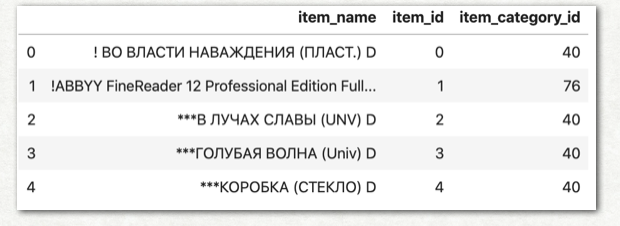
\includegraphics{test.png}
\end{figure}

\subsection{Tables}
\lipsum[12]
See awesome Table~\ref{tab:table}.

\begin{table}
  \caption{Sample table title}
  \centering
  \begin{tabular}{lll}
    \toprule
    \multicolumn{2}{c}{Part}                   \\
    \cmidrule(r){1-2}
    Name     & Description     & Size ($\mu$m) \\
    \midrule
    Dendrite & Input terminal  & $\sim$100     \\
    Axon     & Output terminal & $\sim$10      \\
    Soma     & Cell body       & up to $10^6$  \\
    \bottomrule
  \end{tabular}
  \label{tab:table}
\end{table}

\subsection{Lists}
\begin{itemize}
  \item Lorem ipsum dolor sit amet
  \item consectetur adipiscing elit.
  \item Aliquam dignissim blandit est, in dictum tortor gravida eget. In ac rutrum magna.
\end{itemize}


\bibliographystyle{unsrt}
%\bibliography{references}  %%% Remove comment to use the external .bib file (using bibtex).
%%% and comment out the ``thebibliography'' section.


%%% Comment out this section when you \bibliography{references} is enabled.
\begin{thebibliography}{1}

  \bibitem{kour2014real}
  George Kour and Raid Saabne.
  \newblock Real-time segmentation of on-line handwritten arabic script.
  \newblock In {\em Frontiers in Handwriting Recognition (ICFHR), 2014 14th
      International Conference on}, pages 417--422. IEEE, 2014.

  \bibitem{kour2014fast}
  George Kour and Raid Saabne.
  \newblock Fast classification of handwritten on-line arabic characters.
  \newblock In {\em Soft Computing and Pattern Recognition (SoCPaR), 2014 6th
      International Conference of}, pages 312--318. IEEE, 2014.

  \bibitem{hadash2018estimate}
  Guy Hadash, Einat Kermany, Boaz Carmeli, Ofer Lavi, George Kour, and Alon
  Jacovi.
  \newblock Estimate and replace: A novel approach to integrating deep neural
  networks with existing applications.
  \newblock {\em arXiv preprint arXiv:1804.09028}, 2018.

\end{thebibliography}


\end{document}
